\section{Introduction}
You type a short prompt (``speed up feature computation and make it reproducible'') and the agent returns a 200-line diff: caching layers, parallelized joins, a rewritten pipeline configuration.
You scan the changes in your IDE, hover over a few symbols, run the test suite.
Tests pass; you click Merge.
This is vibe coding~\cite{karpathy2025vibecoding}: you describe intent in natural language, the agent produces code, and you approve based on vibes: surface plausibility rather than structural understanding.
Three months later a regression appears on a demographic slice, and no one can explain why. The structural commitments (e.g., assumptions, dependencies, and trade-offs) behind that diff were never recorded anywhere.
This is not a generation failure. The agent produced correct, executable code.
It is a \emph{control} failure: the system became opaque the moment it was generated.
As projects grow, the practical bottleneck shifts from writing code to understanding and controlling it \cite{peng2023copilot,vaithilingam2022expectation}.
Reviewers cannot determine what invariants were assumed, what dependencies were introduced, or what evidence supports correctness. The agent was not wrong; nothing in the primary artifact encodes this structure.

We call this mismatch the \emph{representation gap}: a system can be executable and pass benchmarks while remaining cognitively inaccessible.
Teams typically respond by imposing process overhead (tickets, documentation, review rituals), but these are external patches on a structural deficiency.
The root cause is \emph{dimension collapse}: the dominant artifact of AI-assisted development (code plus chat history) flattens complex system topology into low-dimensional text, producing systems that are opaque and fragile under change.
The collapse is architectural, and no surface improvement resolves it.
Meaningful control over an AI-generated change requires a reviewer to identify what structural commitments were made, verify their consistency with existing invariants, trace every claim to supporting evidence, and reason about what would break under a different choice.
Code satisfies none of these requirements: structural commitments are implicit in naming and file layout, which agents do not reliably maintain.
Chat history satisfies none of them either; it is a time-ordered negotiation log.
As agent throughput scales and diffs grow larger and more frequent, reviewers are not empowered by better interfaces or more capable models. They are progressively demoted to rubber-stamping opacity. The path forward requires a primary artifact that encodes what code cannot.
\begin{figure}[t]
  \centering
  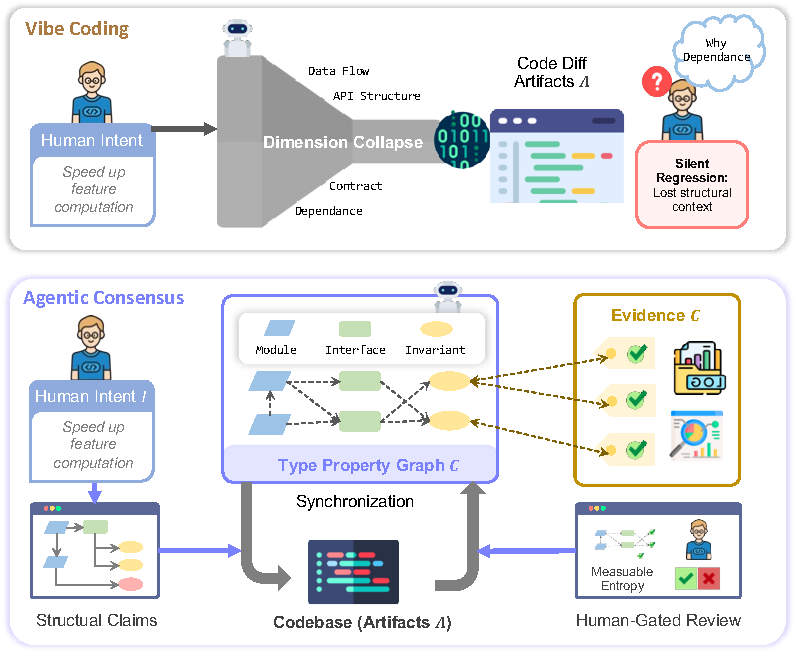
\includegraphics[width=\columnwidth]{figures/consenus-comparison.pdf}
  \caption{Vibe coding (top) treats natural-language prompts as the primary interface and produces code directly, with no persistent structure linking intent to artifacts. Agentic Consensus (bottom) introduces an explicit consensus layer $C$ that mediates between human intent and executable artifacts, maintaining structural traceability and evidence-linked validation throughout the workflow.}
  \label{fig:comparison}
\end{figure}

We propose \textbf{Agentic Consensus} as shown in Figure~\ref{fig:comparison}: a paradigm that replaces ``hoping the AI understood the vibe'' with explicit, operable agreement between humans and machines.
The paradigm shift is to make the consensus layer $C$ the primary artifact of engineering, from which executable artifacts are derived. $C$ is a dynamic, semi-structured operable world model represented as a typed property graph.
Executable artifacts (code, configuration, dataflows) are derived from this shared structure and kept in bi-directional correspondence with it. Linked evidence (tests, checks, traces, provenance) makes every structural claim auditable \cite{chan2024visibility,rasmussen2025zep}.
Programming is thereby reframed as negotiating and validating structural knowledge: entities, dependencies, invariants, and evidence.
The end-state is not ``code that compiles'' but ``structure we agree on.''

\paragraph{Contributions.}
Agentic Consensus is, at its core, a knowledge discovery problem: rehydrating $C$ from artifacts is structure mining; navigating $C$ under uncertainty is graph query answering; evolving $C$ from interaction traces is temporal pattern discovery.
This paper makes four arguments at the intersection of knowledge representation and the emerging challenge of human-AI control:
\begin{itemize}[leftmargin=*, itemsep=2pt]
  \item We argue that the consensus layer $C$ should be the primary artifact of AI-assisted engineering, a structured latent variable mediating between human intent and executable artifacts.
  \item We argue that bidirectional synchronization operators $\Phi$ (realize) and $\Psi$ (rehydrate) are first-class properties that must be continuously executed to maintain consistency between $C$ and $A$
  \item We argue that evaluation must shift from generation quality to alignment and control: alignment fidelity, consensus entropy, intervention distance, and cognitive load reduction.
  \item We propose benchmark task families explicitly designed to measure whether consensus-based workflows reduce human intervention compared to chat-driven baselines.
\end{itemize}

